\section{Methodology}

\begin{frame}{Problem Formulation}
\begin{itemize}

\item Occupancy Map
$$\mathbf{x}^* = \arg\max_{\mathbf{x} \in \mathcal{X}} \sum_{k=1}^{K} \mathcal{M}(T_{\mathbf{x}}\mathbf{s}_k)$$
where $T_{\mathbf{x}}$ is the transformation matrix corresponding to pose $\mathbf{x}$, $\mathcal{M}(\cdot)$ denotes the occupancy function of the map $\mathcal{M}$ at a given point, and $\mathcal{S} = \{\mathbf{s}_k \in \mathbb{R}^3 \mid k = 1, \dots, K\}$ denotes the LiDAR scan.

\item Spatial Hashing Function

\begin{equation*}
    \mathcal{H}_l(\mathbf{v}) =
    \begin{cases}
    1 & \text{if voxel } \mathbf{v} \text{ is occupied}, \\
    0 & \text{otherwise}.
    \end{cases}
\end{equation*}
\end{itemize}
\end{frame}

\begin{frame}{Problem Formulation}
\begin{itemize}

\item Branching
$C_{c_l} = \{ (2x + j_x, 2y + j_y, 2z + j_z, a_\alpha c_\alpha + j_\alpha, a_\beta c_\beta + j_\beta, a_\gamma c_\gamma + j_\gamma, c_{l-1}) \mid{} j_{x, y, z} \in \{0,1\}, j_{\alpha, \beta, \gamma} \in \{0, \ldots{}, a_{\alpha, \beta, \gamma} -1 \} \}
$

where $a_{\alpha, \beta, \gamma}$ are the number of divisions for each rotational component of a node.

\item Score Computation
$$\text{score}(\mathbf{x}) = \sum_{k=1}^{K} \mathcal{H}_l(T_{\mathbf{x}}\mathbf{s}_k)$$
$$\text{score}_{\text{upper}}(c) = \sum_{k=1}^{K} \max_{\mathbf{v} \in \mathcal{N}(T_{\mathbf{x}_c} \mathbf{s}_k)} \mathcal{H}_l(\mathbf{v})$$
where $\mathcal{N}(\cdot)$ denotes the neighborhood voxels surrounding the transformed scan point.

\end{itemize}
\end{frame}

\begin{frame}{Algorithm}
\begin{figure}
    \centering
    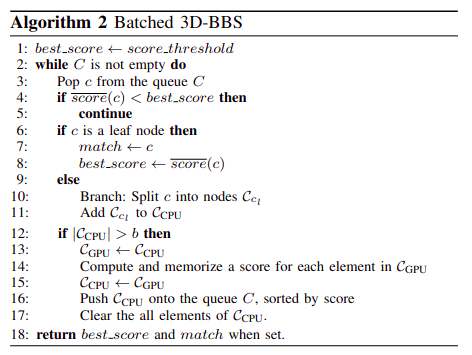
\includegraphics[width=0.75\textwidth]{figures/3dbbs_algorithm.png}
    \caption{3D-BBS Algorithm \cite{aoki20243dbbsgloballocalization3d}}
\end{figure}
\end{frame}

